\documentclass[aps,prx,twocolumn,superscriptaddress,nofootinbib,longbibliography]{revtex4-2}

\usepackage{amsmath,amssymb}
\usepackage{amsthm}
\usepackage{braket}
\usepackage{graphicx}
\usepackage[colorlinks=true,allcolors=blue]{hyperref}

\newtheorem{theorem}{Theorem}
\newtheorem{lemma}{Lemma}

\newcommand{\Ctrue}{C_{\star}}
\newcommand{\xstar}{x_{\star}}
\newcommand{\mean}[1]{\langle #1 \rangle}
\newcommand{\sigA}{\sigma_{A}}
\newcommand{\Tr}{\mathrm{Tr}}
\newcommand{\Dtr}{D_{\mathrm{tr}}}

\begin{document}

\title{A Margolus--Levitin speed limit for observables:\\
mean energy bounds expectation-value change quadratically}

\author{Bryan Nasr}
\email{bryannasr4@gmail.com}
\affiliation{Independent Researcher}

\date{\today}

\begin{abstract}
The Mandelstam--Tamm and Margolus--Levitin quantum speed limits bound how fast a \emph{state}
evolves, using the energy variance and the mean energy above the ground state, respectively. Speed
limits on \emph{observables}---the change of an expectation value $\mean{A(t)}$---have so far used the
energy \emph{variance} (the Mandelstam--Tamm/quantum-Fisher-information lineage); the \emph{mean} energy has
not been brought to bear on the change $\Delta\mean{A}$ in a fixed state. We close this branch. First, we prove a \emph{no-go} theorem: there is no state-independent \emph{linear}
mean-energy bound on the time to change an observable's expectation by $\Delta=|\mean{A(T)}-\mean{A(0)}|$;
the optimal \emph{state-independent} mean-energy exponent of $\Delta$ is exactly two. Second, we prove the corresponding sharp
\emph{quadratic} bound,
$T\,(\mean{H}-E_0)\ge \Ctrue\,\Delta^2/\sigma_A^2$,
valid for every time-independent Hamiltonian $H$ (ground energy $E_0$), every bounded observable $A$ with
spectral spread $\sigma_A=(\lambda_{\max}-\lambda_{\min})/2$, and every pure \emph{or mixed} state, with the
dimension-independent constant $\Ctrue=1/(8\sin \xstar)=0.172506267461\ldots$, where $\xstar$ is the smallest positive
root of $\tan(x/2)=x$. The bound is tight, saturated by a near-ground two-level family. We then promote it to
the \emph{exact} energy--time/swing trade-off curve of which $\Ctrue$ is the small-swing slope---tight at every
swing, the observable analog of the Giovannetti--Lloyd--Maccone curve for states---prove the full constant
survives for mixed states via joint convexity of the trace distance, sharpen the constant for
bandwidth-limited generators and for several observables at once, and show the quadratic law degrades to a
linear one when the initial state is an eigenvector of the observable (a sufficient condition). The result
completes the previously empty (mean-energy $\times$ observable) corner of the speed-limit landscape and, being
quadratic, is most constraining where the linear variance bounds are weakest. We discuss its cleanest physical home---autonomous quantum clocks, where it furnishes a coherent
mean-energy resolution floor complementary to the known entropy and rate bounds---and delimit honestly the
settings it does not constrain.
\end{abstract}

\maketitle

\section{Introduction}
Quantum speed limits (QSLs) quantify how fast a quantum system can change. Two foundational results anchor
the field. The Mandelstam--Tamm (MT) bound~\cite{MandelstamTamm1945} uses the energy \emph{variance}
$\Delta H=\sqrt{\mean{H^2}-\mean{H}^2}$: the time to reach an orthogonal state obeys
$T_\perp\ge \pi/(2\Delta H)$ ($\hbar=1$). The Margolus--Levitin (ML) bound~\cite{MargolusLevitin1998} uses
instead the \emph{mean} energy above the ground state, $T_\perp\ge \pi/[2(\mean{H}-E_0)]$; the two are
unified and tight together~\cite{LevitinToffoli2009}. Both, and the large literature that
followed~\cite{DeffnerCampbell2017}, bound the motion of the \emph{state} (fidelity, Bures angle,
orthogonalization).

A parallel and rapidly growing line bounds the motion of an \emph{observable}---the rate of change of an
expectation value $\mean{A(t)}=\Tr[\rho(t)A]$---which is what an experiment actually
reads~\cite{GarciaPintos2022UnifyingObservables,mohan2022quantum,Bringewatt2024GeneralizedGeometric,Carabba2022operatorflows}.
This program now includes a first-of-kind multiparticle experiment~\cite{Miao2025Experiment}. With few
exceptions, these observable QSLs bound the expectation-value \emph{rate} through the energy \emph{variance}.
The unifying bound of García-Pintos \emph{et al.}~\cite{GarciaPintos2022UnifyingObservables} reads
$|\dot a|\le \Delta A\sqrt{I_F}$ with $I_F$ the quantum Fisher information ($I_F=4\Delta H^2$ for pure
states); Mohan and Pati~\cite{mohan2022quantum} obtain $|\mathrm d\mean{O}/\mathrm dt|\le 2\Delta O\,\Delta H$;
the geometric generalization of Bringewatt \emph{et al.}~\cite{Bringewatt2024GeneralizedGeometric} again
uses the (generalized) Fisher information. All are \emph{linear} in the observable change and powered by an
energy \emph{variance}. The \emph{mean}-energy resource that drives the Margolus--Levitin bound has so far
reached observables only as an \emph{operator}-distance bound for operator
flows~\cite{Carabba2022operatorflows} or through the mean of a transition Hamiltonian for macroscopic
transitions~\cite{Hamazaki2022SpeedLimits}---never as a bound on the change $\Delta\mean{A}$ of a bounded
observable in a fixed state. This is the gap we fill.

We prove that the mean energy controls observable change \emph{quadratically} and not linearly. Concretely
(Sec.~\ref{sec:main}), for a time-independent $H$ with $E_0=\min\mathrm{spec}(H)$, a bounded Hermitian $A$
with spectral spread $\sigma_A=(\lambda_{\max}(A)-\lambda_{\min}(A))/2$, and $\Delta=|\mean{A(T)}-\mean{A(0)}|$,
\begin{equation}
\boxed{\;T\,(\mean{H}-E_0)\;\ge\;\Ctrue\,\frac{\Delta^2}{\sigma_A^2}\;},
\qquad \Ctrue=\frac{1}{8\sin \xstar},
\label{eq:main}
\end{equation}
with $\xstar=2.331122370\ldots$ the smallest positive root of $\tan(x/2)=x$, giving
$\Ctrue=0.172506267461\ldots$. A matching no-go (Sec.~\ref{sec:nogo}) shows no \emph{linear} mean-energy
bound can exist; the quadratic law is the best possible. We then sharpen Eq.~\eqref{eq:main} to the
\emph{exact} tight trade-off curve valid at every swing (Sec.~\ref{sec:constant}). We work in units $\hbar=1$ and, without loss of
generality, shift $E_0=0$ so that $H\succeq0$; $\hbar$ is restored in the applications.

\section{The speed-limit dichotomy}
\label{sec:dichotomy}
The result completes a simple $2\times2$ classification (Table~\ref{tab:dichotomy}), organized by
\emph{what moves} (a state or an observable) and \emph{which energy functional powers the bound} (the
variance or the mean energy).

\begin{table*}[t]
\renewcommand{\arraystretch}{1.6}
\begin{ruledtabular}
\begin{tabular}{lcc}
 & resource $=$ variance $\Delta H$ (Mandelstam--Tamm) & resource $=$ mean energy $\mean{H}-E_0$ (Margolus--Levitin)\\
\hline
state, $1-F$ & $L\le \Delta H\,T$ & $1-F\le K\,T(\mean{H}-E_0)$ \quad (linear)\\
observable, $\Delta\mean{A}$ & $T\ge \Delta/(2\Delta H\,\sigma_A)$ \quad (linear) & $T(\mean{H}-E_0)\ge \Ctrue\,\Delta^2/\sigma_A^2$ \quad \textbf{(quadratic; this work)}\\
\end{tabular}
\end{ruledtabular}
\caption{The speed-limit dichotomy: \emph{what moves} (a state or an observable) $\times$ \emph{which energy
functional} powers the bound (variance or mean energy). Three corners were known; the lower-right
(mean energy $\times$ observable) corner was empty and is the \emph{only} quadratic one.}
\label{tab:dichotomy}
\end{table*}

\noindent Three corners were known; the lower-right (mean energy $\times$ observable) was empty, and it is
the \emph{only} quadratic one. The mechanism is transparent and is the heart of the no-go. The mean energy
bounds only how far the \emph{state} moves---a geometric quantity---through the ML inequality
$1-F\le K\,T(\mean{H}-E_0)$, $F=|\!\braket{\psi(0)|\psi(T)}\!|$. An observable change reads that geometry only
through $\Delta\le 2\sigma_A\sqrt{1-F^2}$, a \emph{square root}. Composing a square root (geometric) with a
linear (energetic) estimate yields $\Delta\propto\sqrt{T(\mean{H}-E_0)}$, i.e.\ a quadratic law. By contrast
MT bounds the observable \emph{velocity} $|\mathrm d\mean A/\mathrm dt|=|\mean{[H,A]}|\le 2\Delta H\,\sigma_A$
directly---no square root---hence linear. (Here $K=\sup_{x>0}(1-\cos x)/x=\sin\xstar$; see
Sec.~\ref{sec:main}.)

\section{No-go: no linear mean-energy bound}
\label{sec:nogo}
\begin{theorem}[No-go]
For time-independent $H$ and bounded Hermitian $A$ there is no positive state-independent constant $\kappa$
with $T(\mean{H}-E_0)\ge \kappa\,\Delta/\sigma_A$ for all $(H,A,\psi)$. More strongly, the sharp
mean-energy bound is quadratic: the exponent of $\Delta$ is exactly $2$.
\end{theorem}
\begin{proof}
By Eq.~\eqref{eq:main}, $P:=T(\mean{H}-E_0)\ge \Ctrue\Delta^2/\sigma_A^2$, and the near-ground two-level
family of Sec.~\ref{sec:constant} saturates it, $P_{\min}(\Delta)=\Ctrue\Delta^2/\sigma_A^2$ as an infimum.
Hence $P_{\min}(\Delta)/(\Delta/\sigma_A)=\Ctrue\,\Delta/\sigma_A\to0$ as $\Delta\to0$: any fixed positive
$\kappa$ is violated by near-ground two-level states. The tight exponent is $2$.
\end{proof}

\noindent The microscopic reason is that $\mean{A(t)}=\sum_{m,n}\overline{c_m}c_n A_{mn}e^{i(E_m-E_n)t}$ is a
\emph{signed} sum over Bohr frequencies weighted by coherences, in contrast to the probability-weighted,
ground-referenced sum $\chi(T)=\sum_n p_n e^{-iE_nT}$ that the mean energy controls. The coherence weight that
sets $\Delta$ and the populations that set $\mean H-E_0$ are independent, which is exactly why a naive linear
transfer of the ML state bound fails.

\section{The sharp quadratic bound}
\label{sec:main}
\begin{theorem}[Main]
Let $H$ be a time-independent Hermitian operator on a finite-dimensional Hilbert space with $E_0=0$
($H\succeq0$), and let $A$ be a bounded Hermitian observable with spectral spread $\sigma_A$. For any pure
state, with $\Delta=|\mean{A(T)}-\mean{A(0)}|$,
\begin{equation}
T\,\mean{H}\;\ge\;\Ctrue\,\frac{\Delta^2}{\sigma_A^2},\qquad \Ctrue=\frac{1}{8K},\quad K=\sup_{x>0}\frac{1-\cos x}{x}.
\end{equation}
\end{theorem}

\begin{proof}
Work in the energy eigenbasis, $\ket{\psi}=\sum_n c_n\ket n$, $p_n=|c_n|^2$. Both sides scale as
$\sigma_A^2$, and $\Delta$ and the dynamics of $\mean{A(t)}$ are invariant under $A\to A+cI$ (since
$\Tr[\rho_T-\rho_0]=0$); center $A$ so that $\|A\|_{\mathrm{op}}=\sigma_A$ and set $\sigma_A=1$.

\emph{Step 1 (geometry).} With $\rho_t=\ket{\psi(t)}\!\bra{\psi(t)}$ and $X=\rho_T-\rho_0$ (traceless,
Hermitian), Hölder's inequality gives $\Delta=|\Tr[AX]|\le\|A\|_{\mathrm{op}}\|X\|_1=\|X\|_1$. For two pure
states the nonzero eigenvalues of $X$ are $\pm\sqrt{1-F^2}$, $F=|\!\braket{\psi(0)|\psi(T)}\!|$, so
$\|X\|_1=2\sqrt{1-F^2}$ and
\begin{equation}
\Delta\le 2\sqrt{1-F^2}.
\label{eq:step1}
\end{equation}

\emph{Step 2 (energetics).} The survival amplitude is $\chi(T)=\sum_n p_n e^{-iE_nT}$ and $F\ge\mathrm{Re}\,\chi(T)$.
By the tangent-line lemma below, $1-\cos x\le Kx$ for all $x\ge0$, so
\begin{equation}
1-F\le 1-\mathrm{Re}\,\chi(T)=\sum_n p_n(1-\cos E_nT)\le K\,T\mean{H}.
\label{eq:step2}
\end{equation}

\emph{Combine.} $1-F^2=(1-F)(1+F)\le 2(1-F)\le 2KT\mean H$. Inserting into \eqref{eq:step1},
$\Delta^2\le 4(1-F^2)\le 8KT\mean H$, i.e.\ $T\mean H\ge \Delta^2/(8K)=\Ctrue\Delta^2$ (with $\sigma_A=1$).
Restoring $\sigma_A$ gives the claim. Retaining the exact geometry $1-F\ge1-\sqrt{1-\delta^2}$
($\delta=\Delta/2\sigma_A$) before the step $1-F^2\le2(1-F)$ yields the sharper non-asymptotic form
$T\mean H\ge(1-\sqrt{1-\delta^2})/K$, whose leading term is $\Ctrue\Delta^2/\sigma_A^2$ and which is strictly
stronger for every finite $\delta$ (by a factor approaching $2$ as $\delta\to1$).
\end{proof}

\noindent The energetics (Step~2)---ground-referencing $H$, the survival amplitude $\chi(T)$, and the
eigenbasis cosine estimate---follows the statistical-distance derivation of the Margolus--Levitin bound by
Jones and Kok~\cite{JonesKok2010GeometricDerivation} (corrected by Zwierz~\cite{Zwierz2012Comment}) and the
survival-amplitude inequality of Bhattacharyya~\cite{Bhattacharyya1983}; the new step is to place a bounded
observable on the left via Hölder (Step~1), converting the state-distance bound into one on $\Delta\mean{A}$.
Since $\chi(T)$ contains only populated levels, the bound also holds with $\mean H$ referenced to the lowest
\emph{populated} energy $E_{\min}^{\mathrm{supp}}\ge E_0$, a state-dependent strengthening.

\begin{lemma}[Tangent line]
$K:=\sup_{x>0}(1-\cos x)/x$ is attained at the unique stationary point $\xstar$ of $(1-\cos x)/x$ in
$(0,2\pi)$---equivalently, the smallest positive root of $x\sin x=1-\cos x\Leftrightarrow\tan(x/2)=x$---and
$K=\sin\xstar$. The line $y=Kx$ is tangent to $1-\cos x$ at $\xstar$ and lies above it for all $x\ge0$, with
equality only at $x=0$ and $x=\xstar$.
\end{lemma}

\noindent This tangent-line constant is the orthogonality ($q\to0$) member of the generalized
Margolus--Levitin construction of Giovannetti, Lloyd, and Maccone~\cite{Giovannetti2003QuantumLimits}; the
same $K\approx0.7246$ underlies the operator-flow bound of Ref.~\cite{Carabba2022operatorflows}. Applying the
theorem to $E_{\max}I-H\succeq0$ (which shares $F$, $\sigma_A$, and $\Delta$) gives the ceiling-referenced
companion $T\,(E_{\max}-\mean H)\ge\Ctrue\Delta^2/\sigma_A^2$ with the \emph{same} constant; combined,
$T\ge\Ctrue\Delta^2/[\sigma_A^2\min(\mean H-E_0,\,E_{\max}-\mean H)]$---the observable analog of the
bounded-spectrum (dual) Margolus--Levitin bound~\cite{Ness2022BoundedSpectrumQSL}, whose floor is weakest at
mid-spectrum and does not vanish as $\mean H$ grows. The proof uses only the pointwise tangent inequality and a
finite mean energy, so it extends to a separable infinite-dimensional Hilbert space with bounded $A$ and a
spectral measure of finite first moment.

\noindent Figure~\ref{fig:tangent} shows the lemma. All inequalities are elementary and exact; we verified
the chain numerically over $10^5$ random configurations in dimensions $2$--$7$ with zero violations
(Sec.~\ref{sec:numerics}).

\begin{figure}[t]
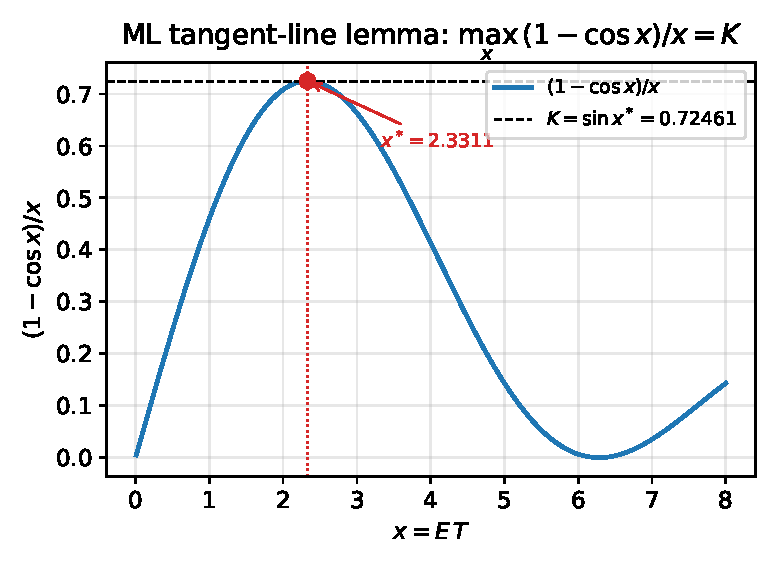
\includegraphics[width=\columnwidth]{figs/fig2_tangent.pdf}
\caption{The tangent-line lemma. $(1-\cos x)/x$ attains its supremum $K=\sin\xstar=0.724611\ldots$ at
$\xstar=2.331122\ldots$ (root of $\tan(x/2)=x$), which fixes the sharp constant $\Ctrue=1/(8K)$.}
\label{fig:tangent}
\end{figure}

\section{Exact constant, trade-off curve, and saturation}
\label{sec:constant}
The constant admits several equivalent closed forms,
\begin{equation}
\Ctrue=\frac{1}{8K}=\frac{1}{8\sin\xstar}=\frac{\xstar}{8(1-\cos\xstar)}=\frac{1+\xstar^2}{16\,\xstar},
\end{equation}
all equal to $0.172506267461\ldots$ and agreeing to $52$ digits (\texttt{mpmath}). It is dimension-independent and \emph{sharp}: it is approached,
though not attained, by the near-ground two-level family
$H=\mathrm{diag}(0,E)$, $A=\sigma_x$ ($\sigma_A=1$),
$\ket{\psi}=\cos\theta\ket0+\sin\theta\,e^{i\beta}\ket1$, in the limit $\theta\to0$ with $ET=\xstar$ and the
\emph{optimal relative phase} $\beta=\xstar/2-\pi/2$ (which starts $\mean{A(t)}$ at maximum slope rather than
at a turning point). There all three inequalities saturate simultaneously. A dedicated global optimizer over
$(E_n,A,\psi)$ in $d=2$--$10$ confirms the floor: the smallest ratio found is
$0.172506558\ge\Ctrue$, approached from above as $\theta\to0$, and no configuration dips below
(Fig.~\ref{fig:multid}). Phase restriction ($\beta=0$, real amplitudes) gives instead the strictly larger
$C_{\beta=0}=\dfrac{1}{16\,\phi_\star\sin^2\phi_\star}=\dfrac{\phi_\star}{4(1-\cos\phi_\star)^2}=0.185551\ldots$
($+7.6\%$), with $\phi_\star=2.78650\ldots$ the smallest positive root of $1-\cos x=2x\sin x$, saturated at the
turning-point configuration; the optimal relative phase recovers the full factor (Fig.~\ref{fig:converge}).

\medskip
\noindent\emph{The complete trade-off curve.} The constant $\Ctrue$ is the $\delta\to0$ slope of a sharp
\emph{curve}. With budget $P=T(\mean H-E_0)$ and normalized swing $\delta=\Delta/2\sigma_A\in[0,1)$, the
minimum budget that produces swing $\delta$---over all $(H,A,\rho,d,T)$---is
$P_\star(\delta)=\min\{T(\mean H-E_0):\Delta/2\sigma_A=\delta\}$, attained on a two-level Bohr-active subspace
and given parametrically in the Bohr phase $\tau=ET\in[\xstar,\pi)$ by
\begin{equation}
\begin{gathered}
\sin^2\theta=\frac{\tau-\tan(\tau/2)}{\tau-2\tan(\tau/2)},\qquad P_\star=\tau\sin^2\theta,\\[2pt]
\delta=\sin2\theta\,\sin(\tau/2),\qquad \tau=ET\in[\xstar,\pi).
\end{gathered}
\label{eq:curve}
\end{equation}
It interpolates from $P_\star(\delta)=4\Ctrue\delta^2[1+O(\delta^2)]$ as $\delta\to0$ (recovering the constant)
to $P_\star\to\pi/2$ as $\delta\to1$ (Fig.~\ref{fig:curve}), lying strictly above the elementary bound
$(1-\sqrt{1-\delta^2})/K$ of Sec.~\ref{sec:main}---by $1.3\%$ at $\delta=0.5$, $4.2\%$ at $\delta=0.8$, $8.2\%$
at $\delta=0.95$, but under $1\%$ in the near-ground window where the applications operate. The curve is the
\emph{observable image} of the Giovannetti--Lloyd--Maccone state trade-off: $\Delta=2\sigma_A\sqrt{1-F^2}$ is
saturable (align the $\pm\sigma_A$ eigenvectors of $A$ with the rank-two $\rho_T-\rho_0$), so the maximal swing
at fixed budget is $2\sigma_A\sqrt{1-F_{\min}^2}$ with $F_{\min}$ the minimal survival fidelity at fixed mean
energy~\cite{Giovannetti2003QuantumLimits}, whose two-level
optimizer~\cite{Hornedal2023MargolusLevitinArbitraryFidelity} carries over; a multi-start search over
$d=2$--$6$ finds no state below $P_\star(\delta)$ at any $\delta$. This is the observable counterpart---tight at
every $\delta$, not only in the constant---of the exact arbitrary-fidelity Margolus--Levitin curve for states.

\medskip
\noindent\emph{Bandwidth-resolved constant.} If $\mathrm{spec}(H)\subset[E_0,E_0+B]$, the tangent-line
supremum runs only over $x\in(0,BT]$, so $K\to K(L)=\sup_{0<x\le L}(1-\cos x)/x$ with $L=BT$. Since
$(1-\cos x)/x$ increases on $(0,\xstar)$, $K(L)=(1-\cos L)/L$ for $L<\xstar$ and $K(L)=K$ otherwise, giving the
spectrally sharp constant
\begin{equation}
\Ctrue(L)=\frac{1}{8K(L)},\qquad T(\mean H-E_0)\ge \Ctrue(BT)\,\frac{\Delta^2}{\sigma_A^2},
\label{eq:bandwidth}
\end{equation}
which recovers $\Ctrue$ for $L\ge\xstar$ and is strictly stronger for narrow-band, short-time operation
($1.58\times$ at $L=1$, $2.96\times$ at $L=0.5$), saturated by a two-level gap at the band edge---sharpening
the floor for precisely the low-bandwidth devices (e.g.\ minimal clocks) where the bound is most relevant.

\begin{figure}[t]
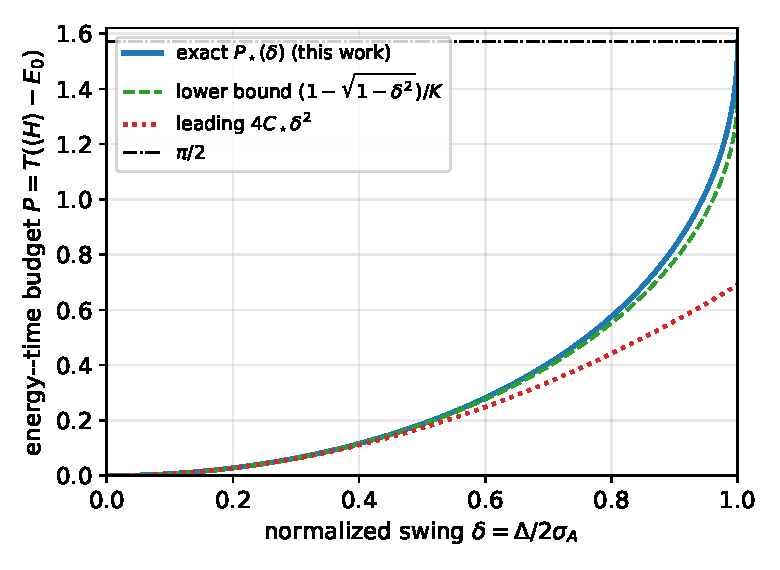
\includegraphics[width=\columnwidth]{figs/fig5_curve.pdf}
\caption{The exact observable trade-off curve $P_\star(\delta)$, Eq.~\eqref{eq:curve}: the minimum energy--time
budget $P=T(\mean H-E_0)$ for a normalized swing $\delta=\Delta/2\sigma_A$, tight at every $\delta$. Its slope
as $\delta\to0$ is set by $\Ctrue$ and its $\delta\to1$ limit is $\pi/2$. It lies above the elementary lower
bound $(1-\sqrt{1-\delta^2})/K$ and its leading term $4\Ctrue\delta^2$.}
\label{fig:curve}
\end{figure}

\begin{figure}[t]
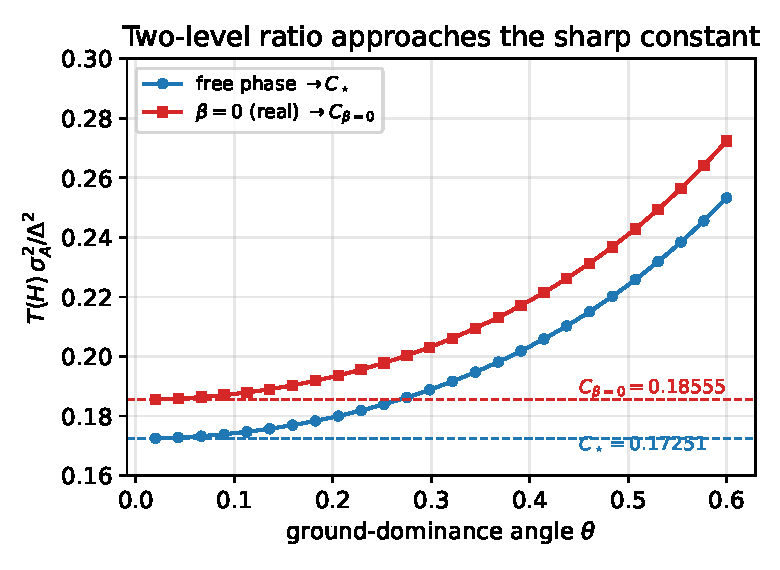
\includegraphics[width=\columnwidth]{figs/fig1_convergence.pdf}
\caption{The two-level ratio $T\mean{H}\sigma_A^2/\Delta^2$ versus the ground-dominance angle $\theta$,
approaching the sharp constant $\Ctrue$ (free relative phase) and the phase-restricted suboptimum
$C_{\beta=0}=0.185551$, both from above as $\theta\to0$.}
\label{fig:converge}
\end{figure}

\begin{figure}[t]
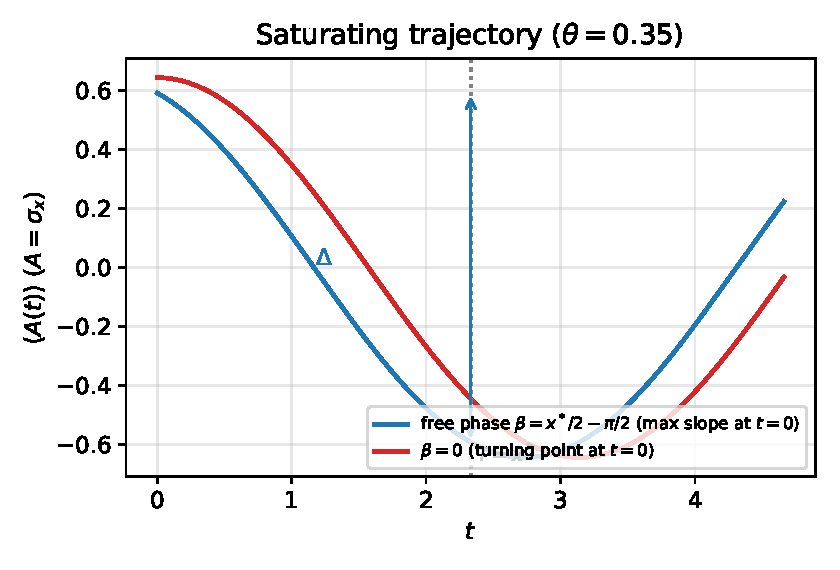
\includegraphics[width=\columnwidth]{figs/fig3_trajectory.pdf}
\caption{Saturating trajectory $\mean{A(t)}$ ($A=\sigma_x$). With the optimal phase the expectation starts at
maximum slope (and reaches its excursion $\Delta$ at $T=\xstar/E$); the real-amplitude ($\beta=0$) case starts
at a turning point and is suboptimal.}
\label{fig:traj}
\end{figure}

\begin{figure}[t]
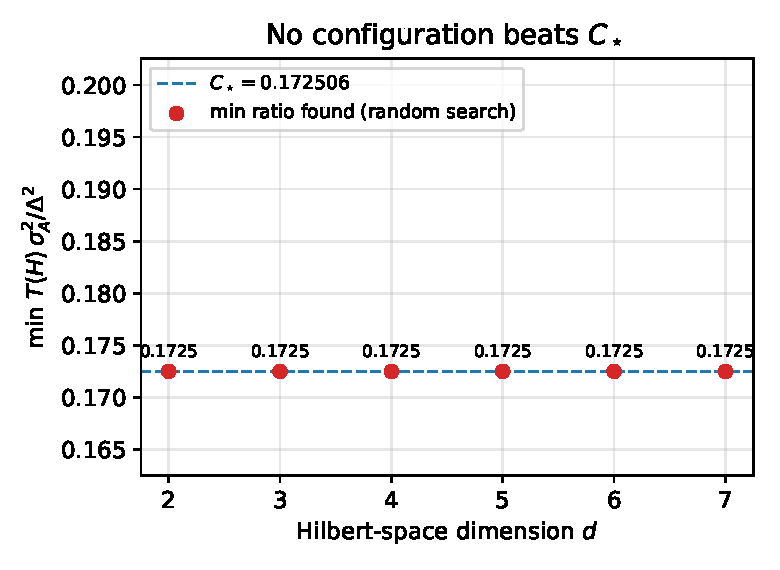
\includegraphics[width=\columnwidth]{figs/fig4_multid.pdf}
\caption{Global-optimizer minimum of $T\mean{H}\sigma_A^2/\Delta^2$ per Hilbert-space dimension $d$.
No configuration in $d=2$--$7$ beats $\Ctrue$; each dimension approaches it from above.}
\label{fig:multid}
\end{figure}

\section{Mixed states and normalization}
\label{sec:mixed}
The bound holds for an arbitrary density matrix $\rho_0$ \emph{with the same constant} $\Ctrue$, with
$\rho_T=U\rho_0U^\dagger$, $U=e^{-iHT}$, $\Delta=|\Tr[A(\rho_T-\rho_0)]|$, $\mean{H}=\Tr[\rho_0H]$.
The geometric step generalizes via Hölder to $\Delta\le 2\sigma_A\Dtr(\rho_0,\rho_T)$, with $\Dtr$ the trace
distance. The key is to avoid an Uhlmann-fidelity detour (which loses a factor of two) by using
\emph{joint convexity} of the trace distance on the spectral decomposition $\rho_0=\sum_k p_k\ket k\!\bra k$:
since the \emph{same} $U$ evolves every eigenvector, $\rho_T=\sum_k p_k\,U\ket k\!\bra k U^\dagger$ is a convex
combination with the \emph{identical} weights $p_k$, so
\begin{equation}
\Dtr(\rho_0,\rho_T)\le\sum_k p_k\sqrt{1-F_k^2},\qquad F_k=|\!\braket{k|U|k}\!|.
\end{equation}
Per-eigenstate ML gives $1-F_k\le K T\,e_k$ with $e_k=\braket{k|H|k}\ge0$, and Jensen's inequality (concavity
of $\sqrt{\cdot}$, $\sum_k p_k e_k=\mean H$) yields
$\sum_k p_k\sqrt{2KTe_k}\le\sqrt{2KT\mean H}$. Combining,
$\Delta\le 2\sigma_A\sqrt{2KT\mean H}$, hence $T\mean H\ge\Ctrue\Delta^2/\sigma_A^2$. The same constant
follows independently by purification ($H\!\otimes\!I$, $A\!\otimes\!I$ preserve $\mean H$, $\sigma_A$ and
$\Delta$ exactly, so the pure bound descends). Each inequality is strict away from the pure $\theta\to0$ limit,
so every state with $\Delta>0$ lies strictly above $\Ctrue$; yet $\Ctrue$ remains the tight infimum for mixed
states as well (no pure/mixed gap), approached by mixing the saturating family with a vanishing ground-state
weight, consistent with the saturation analysis of Ref.~\cite{Sonnerborn2026MLsaturate}.

Among candidate normalizations, the spectral spread $\sigma_A=(\lambda_{\max}-\lambda_{\min})/2$ is canonical:
it is the Chebyshev radius $\min_c\|A-cI\|_{\mathrm{op}}$, which makes the Hölder step tight; it is
shift-invariant and state-independent. The operator norm $\|A\|_{\mathrm{op}}\ge\sigma_A$ gives a weaker valid
bound, while the state variance $\Delta A_\rho\le\sigma_A$ (Popoviciu) is the variance scale of the MT family
and is not delivered by this proof.

\medskip
\noindent\emph{Several observables at once.} Because the bound depends on the state only through
$X=\rho_T-\rho_0$, it constrains a whole family $\{A_i\}$ jointly: for any real combination $A_u=\sum_iu_iA_i$
with swing $\Delta_u=|\Tr[A_uX]|$ and Chebyshev radius $\|A_u\|_{\mathrm{Cheb}}$, Step~1 gives
$\Delta_u\le\|A_u\|_{\mathrm{Cheb}}\,2\sqrt{1-F^2}$, hence
\begin{equation}
T(\mean H-E_0)\ge \Ctrue\,\sup_{u}\frac{\Delta_u^2}{\|A_u\|_{\mathrm{Cheb}}^2},
\label{eq:multi}
\end{equation}
a mean-energy bound set by the operator-norm (Chebyshev) \emph{dual} geometry, in contrast to the Fisher-metric
multiparameter variance limits~\cite{Hamazaki2023QuantumVelocityLimits,Bringewatt2024GeneralizedGeometric}. For
two orthonormal observables (e.g.\ $\sigma_x,\sigma_y$) it reads
$T(\mean H-E_0)\ge\Ctrue(\Delta_1^2+\Delta_2^2)/\sigma_A^2$, twice the single-observable floor when
$\Delta_1=\Delta_2$.

\section{Structure: linear recovery and structured observables}
\label{sec:structure}
The quadratic law is a property of \emph{generic} observables, whose expectation starts at maximum slope. It
degrades to a \emph{linear} law when the initial state is an eigenvector of $A$ (a sufficient condition).
\begin{theorem}[Linear recovery]
If $A\ket{\psi_0}=\lambda\ket{\psi_0}$, then with $l=(\lambda-\mathrm{center}(\mathrm{spec}\,A))/\sigma_A\in[-1,1]$,
\begin{equation}
T\,(\mean{H}-E_0)\ge\frac{1}{2K(1+|l|)}\,\frac{\Delta}{\sigma_A},
\end{equation}
sharpest at an extreme eigenvalue ($|l|=1$): $T(\mean{H}-E_0)\ge \Delta/(4K)=2\Ctrue\,\Delta/\sigma_A$.
\end{theorem}
\begin{proof}
Center $A$, $\sigma_A=1$; set $B=A-\lambda I$, so $B\ket{\psi_0}=0$. Writing
$\ket{\psi_T}=e^{i\alpha}F\ket{\psi_0}+\sqrt{1-F^2}\ket{\phi}$ with $\ket\phi\perp\ket{\psi_0}$, the cross
terms vanish ($B\ket{\psi_0}=0$, $B$ Hermitian), so $\Delta=(1-F^2)|\!\braket{\phi|B|\phi}\!|\le(1+|l|)(1-F^2)$
---linear in the fidelity deficit. With $1-F^2\le2(1-F)\le2KT\mean H$ the claim follows.
\end{proof}
\noindent Thus a fidelity-aligned observable such as the projector $\ket{\psi_0}\!\bra{\psi_0}$ literally
reduces the bound to the linear ML \emph{state} bound (then $\mean{A(t)}=F^2$, $\Delta=1-F^2$), recovering the
upper-right corner of the dichotomy. We emphasize that a turning point alone (zero initial slope without
$\ket{\psi_0}$ being an eigenvector) is \emph{not} sufficient: e.g.\ $\ket{\psi_0}=(\ket0+\ket1)/\sqrt2$,
$A=\mathrm{diag}(1,-1,0)$, $H$ with real $H_{01}$ has zero initial slope yet no positive linear constant
($r_{\mathrm{lin}}$ falls to $\approx0.03\ll1/4K$).

For structured observables the constant does not improve generically: a rank-one ground coupling
$A=\ket0\!\bra v+\ket v\!\bra0$ still gives $\inf=\Ctrue$ (the saturating family is itself of this form), and
an energy-banded ground-touching $A$ likewise. Restricting to real couplings and amplitudes raises the
constant to $C_{\beta=0}=0.185551$. A ground-decoupled observable ($A_{0n}=0$) conserves the excited
population and makes the time bound vacuous; a static energy floor $\mean H-E_0\ge(\Delta_{\mathrm{gap}}/2)\Delta/\sigma_A$
governs instead. The bound is informative for observables of finite spectral spread (spins, parity,
projectors, qubit registers); for unbounded observables ($\sigma_A=\infty$, e.g.\ position or particle number)
it is vacuous, and Mandelstam--Tamm, which uses the finite state variance, is operative.

\section{Numerical verification}
\label{sec:numerics}
All numerics are seeded and reproducible (\texttt{numerics/}; consolidated in
\texttt{results.json}). The named constant is pinned to $52$ digits with \texttt{mpmath}. The no-go exponent
is confirmed by the log--log slope of $P_{\min}(\Delta)$ along the saturating family ($2.0$). The pure-state
bound survives $10^5$ random trials in $d=2$--$7$ (worst-case slacks $\ge0$ to machine precision) and a
dedicated multi-start optimizer (Fig.~\ref{fig:multid}); the apparent sub-$\Ctrue$ minima are floating-point
catastrophic cancellation at excited population $\sim10^{-14}$ and disappear at $60$-digit precision. The
mixed-state bound is confirmed by a violation search over random density matrices (minimum sampled ratio
$0.176\ge\Ctrue$) and by a direct audit of the convexity chain; the infimum over mixed states is again
$\Ctrue$, approached as the state purifies onto the saturating family. The linear-recovery constant $1/4K$ and the structured constants $\Ctrue$, $C_{\beta=0}$ are
reproduced to six digits. The exact trade-off curve $P_\star(\delta)$ is confirmed as a strict lower boundary
by a multi-start search in $d=2$--$6$ (no state dips below it at any $\delta$); the bandwidth-resolved bound
$\Ctrue(BT)$ by a violation search over spectrally bounded $H$ ($0$ violations in $1.5\times10^5$ trials); and
the two-observable bound saturates the $2\times$ gain at $\Delta_1=\Delta_2$.

\section{Applications and discussion}
\label{sec:apps}
The most important consequence is structural: Eq.~\eqref{eq:main} is the first mean-energy, quadratic-in-$\Delta$
member of the observable-QSL family, the variance/Fisher members being \emph{linear} in
$\Delta$~\cite{GarciaPintos2022UnifyingObservables,mohan2022quantum,Bringewatt2024GeneralizedGeometric}.
Being quadratic, it is most constraining exactly where the linear bounds are weakest---for \emph{large}
fractional changes $\Delta/\sigma_A$---so the two families are complementary, not competing. Observable QSLs
are an active, growing area, including recent experiments~\cite{Miao2025Experiment}.

\paragraph{A regime where the bound binds.}
There is an identifiable window in which Eq.~\eqref{eq:main} is the operative observable limit. For the
near-ground qubit $H=\tfrac\omega2\sigma_z$, $A=\sigma_x$,
$\ket{\psi_0}=\sqrt{1-\varepsilon}\,\ket g+\sqrt\varepsilon\,\ket e$ (excited population $\varepsilon$, ground
state $\ket g$) evaluated at the half-period $T_\star=\pi/\omega$, the mean-energy floor exceeds the
Mandelstam--Tamm observable floor $\Delta/(2\Delta H\sigma_A)$ by the exact factor $8\Ctrue(1-\varepsilon)$,
which is $>1$ for ground dominance $\varepsilon<0.275$. There---small excited population, large fractional
swing---the quadratic mean-energy bound, not the variance bound, sets the limit. Read in reverse,
an observed swing $\Delta$ over time $T$ \emph{certifies} a mean energy $\mean H-E_0\ge\Ctrue\Delta^2/(\sigma_A^2T)$
from a single bounded-observable expectation, with no state-overlap measurement. With $\hat\Delta$ estimated
from finite samples (standard error $s$), error propagation gives the one-sided certificate
$\mean H-E_0\ge\Ctrue[\max(0,\hat\Delta-z_\alpha s)]^2/(\sigma_A^2T)$ at confidence $1-\alpha$---a
model-independent energy floor measurable on the platforms now realizing observable speed
limits~\cite{Miao2025Experiment}, in the regime above where it binds.

\paragraph{Autonomous quantum clocks (primary).}
An autonomous clock is by definition driven by a fixed, time-independent
Hamiltonian~\cite{Erker2017AutonomousClocks,Woods2021AutonomousTicking}, so the hypotheses of
Eq.~\eqref{eq:main} hold exactly. Taking $A$ to be the clock's bounded pointer (hand) observable and $\Delta$
a resolvable advance, the bound becomes a coherent \emph{resolution floor},
\begin{equation}
T_{\mathrm{res}}\;\ge\;\hbar\,\Ctrue\,\frac{\Delta^2}{(\mean{H}-E_0)\,\sigma_A^2},
\end{equation}
i.e.\ the mean energy stored in the clockwork lower-bounds the time to move the hand by a resolvable amount.
A precessing pointer ($H=\tfrac\omega2\sigma_z$, $A=\sigma_x$) obeys it, with the bound tightest for the
smallest, lowest-energy ``minimal'' clock; saturation is a near-ground limit, and at its natural (equatorial)
operating point the pointer is an $A$-turning point---the linear regime of Sec.~\ref{sec:structure}---so it
illustrates rather than saturates the quadratic floor. This complements---rather than subsumes---the
established clock limits, which use \emph{different} resources: dissipated entropy per tick
($N\lesssim\Delta S_{\mathrm{tick}}/2k_B$)~\cite{Erker2017AutonomousClocks,Pearson2021Timekeeping} and the
thermalization rate ($N\le\Gamma^2/\nu^2$)~\cite{Meier2023AccuracyResolution}, both for open dissipative
clocks. Mean energy alone does not \emph{upper}-bound clock or computational speed~\cite{Jordan2017FastComputation};
ours is a complementary lower bound at fixed pointer contrast $\sigma_A$.

\paragraph{Autonomous quantum batteries (secondary).}
For an autonomous (time-independent generator) battery with $A=H_B$ the stored energy, $\Delta=W$ the energy
deposited, and $\sigma_B$ the battery's spectral spread, Eq.~\eqref{eq:main} gives a minimum charging time
$T_{\min}=\hbar\Ctrue W^2/[(\mean{H_{\mathrm{tot}}}-E_0)\sigma_B^2]$, quadratic in $W$. This is a
\emph{complementary} mean-energy floor: mainstream charging is driven by time-dependent control and its
operative power bounds are variance/Fisher
based~\cite{GarciaPintos2020BatteryPower,JuliaFarre2020Battery,Campaioli2024Colloquium} (the García-Pintos
bound has a published correction~\cite{Cusumano2021Comment}), and the reported quantum advantage stems from
super-extensive \emph{variance}, not mean energy. The same algebra rearranges into an energetic-cost floor on
changing a logical observable in any always-on (autonomous) architecture; it is, however, loose for typical
fast gates, and standard time-dependent gate pulses fall outside the hypotheses. Because $\sigma_B$ tracks the
battery bandwidth, this floor falls as $1/N$ for an $N$-cell battery and sits a fixed factor below the
Margolus--Levitin charging time even at $N=1$, and it bounds the deposited energy $W$ rather than the
ergotropy~\cite{Shrimali2024StrongerSpeedLimit}; we therefore offer it as an illustrative remark, not a
binding constraint.

\paragraph{What the bound does not constrain.}
Honesty about scope sharpens the claim. (i) Standard, time-dependently driven quantum gates violate the
time-independence hypothesis---essential here, since the Margolus--Levitin bound provably does not extend to
closed systems with time-dependent generators~\cite{Hornedal2023ClosedSystems,Hornedal2023MargolusLevitinArbitraryFidelity}. (ii) For extensive many-body systems the total mean energy grows like the
system size, so the bound is weak for \emph{local} observables; there the operative limit is locality-based
(Lieb--Robinson)~\cite{Chen2023LocalitySpeedLimits}. (iii) In quantum metrology/sensing the operative speed
limit is the variance (MT) one and practical readout times are set by signal-to-noise and decoherence far
above any mean-energy floor~\cite{HerbDegen2024Sensing}; the bound nonetheless lower-bounds the mean-energy
\emph{cost} of generating a given signal swing, complementing the asymmetry/weak-value observable speed limit
of Budiyono \emph{et al.}~\cite{Budiyono2026QSLObservables}. The bound is therefore a statement about
energy-constrained, few-body or near-ground dynamics.

\paragraph{Outlook.}
Natural extensions are open-system (Lindbladian) and time-dependent-$H$ generalizations---where much of the
driven-application landscape lives---and a sharp constant for ergotropy rather than stored energy. Within the
present setting, the constant sharpens under a spectral-bandwidth restriction
($K\to\sup_{0<x\le BT}(1-\cos x)/x$) and generalizes to higher energy moments~\cite{ChauZeng2024UnifyingQSL}, and the bound assembles with the
observable Mandelstam--Tamm limit into a unified envelope
$T\ge\max[\,\Delta/(2\Delta H\sigma_A),\,\Ctrue\Delta^2/((\mean H-E_0)\sigma_A^2)\,]$ in the spirit of
Levitin--Toffoli~\cite{LevitinToffoli2009} and the bounded-spectrum treatment~\cite{Ness2022BoundedSpectrumQSL}.

\section{Conclusion}
We have established the missing mean-energy speed limit for observables: a no-go against any linear law and a
sharp quadratic bound $T(\mean{H}-E_0)\ge\Ctrue\Delta^2/\sigma_A^2$ with a closed-form, dimension-independent
constant, valid for pure and mixed states, tight, and degrading to a linear law for eigenvector observables.
Beyond the constant we gave the complete, tight trade-off curve $P_\star(\delta)$ (the observable analog of the
arbitrary-fidelity Margolus--Levitin curve), its bandwidth-resolved and multi-observable refinements, and its
backward reading as a model-independent mean-energy certificate. Together these make the
(mean-energy $\times$ observable) corner of the speed-limit dichotomy a complete and operationally grounded
one; its cleanest physical home is the thermodynamics of timekeeping.

% \begin{acknowledgments}
% Add acknowledgments here before submission.
% \end{acknowledgments}

\bibliography{refs}

\end{document}
